\documentclass[a4paper]{article}
\usepackage{graphicx} % Required for inserting images
\usepackage{dcolumn}
\usepackage{tabularx}
% \usepackage[style=authoryear]{biblatex}
\usepackage[style=authoryear, backend=biber, hyperref=true, parentracker=true]{biblatex}
\usepackage[colorlinks=true]{hyperref}
\usepackage[margin=1in]{geometry}

\addbibresource{references.bib}
\title{Uncovering the impact of texts in the cover images of crowdfunding campaigns}
\author{}
\date{May 5, 2024}

\begin{document}

\maketitle


\begin{abstract}
    Incorporating text into images is popular in crowdfunding campaigns. Studies have shown that the aesthetic features of images of a campaign are critical for the campaign's success, but how text inclusion in campaign images affects campaign attractiveness is still under limited study. To fill the research gap, this paper aims to explore the impact of text in the cover image of a campaign on the campaign's attractiveness.  Using datasets from a leading crowdfunding platform in China, we discovered that incorporating text into the cover image of a campaign could significantly improve the campaign's attractiveness, and the impact of text density on campaign attractiveness is in an inverse U shape. We also discovered that text in the center of an image could be more attractive. Such findings are also confirmed by a series of experiments. 
\end{abstract}

\tableofcontents

\section{Introduction}
It is becoming popular to incorporate text into images in crowdfunding campaigns. On one hand, such text could enrich the information contained in the image, while on the other hand, such text would require more recognition resources to process such information, leading to the phenomenon of information overload. This paper aims to study the impact of text incorporation in the campaign's cover image on the campaign's attractiveness. Specifically, we study the following three questions?
\begin{enumerate}
    \item Does text in the cover image could increase the campaign's attractiveness?
    \item What is the relationship between text density in the cover image and the campaigns' attractiveness?
    \item Will the position of the text in the cover image affect the campaign's attractiveness?
\end{enumerate}

The contributions of the paper are as follows.
\begin{enumerate}
    \item This is one of the pioneering studies that examine the impact of text in images on crowdfunding campaign attractiveness. 
    \item This paper sheds light on the intriguing relationship between image-text combination and human recognition.
    \item This paper put forward new ideas to conduct experiments with the help of state-of-the-art AI technologies such as ChatGPT. 
      
\end{enumerate}

\section{Literature review}
\subsection{Crowdfunding}
Crowdfunding, a compound term composed of “crowd” and “funding”, is a financing method that raises small amounts of fundings from a large number of individuals(i.e.,“the crowd”) via an internet platform to fund startup entrepreneurs(Mollick, 2014).Typically, entrepreneurs offer products or equity as returns to individuals. Based on the type of return provided, crowdfunding can be categorized into four types: equity-based crowdfunding, loan-based crowdfunding, donation-based crowdfunding, and reward-based crowdfunding(Burtch et al., 2013;Belle et al., 2015).Equity-based crowdfunding refers to a financing method in which the fundraiser offers a certain proportion of shares, giving investors the opportunity to become shareholders in the project and enjoy future profits(Vismara, 2015). In loan-based crowdfunding, participants provide funds to the project initiator in the form of a loan, requiring the initiator to repay the principal and interest within a specified future timeframe. Reward-based crowdfunding commonly rewards supporters with non-monetary rewards, products, or services in return for their support. In contrast, donation crowdfunding, unlike the other three types, does not require any form of return(Xu, 2018). This study takes the example of the Modian website, a reward-based crowdfunding platform. Cumming et al. categorized reward-based crowdfunding into two models, “Keep-It-All”(KIA) and “All-Or-Nothing”(AON), based on the fundraising goals set by entrepreneurs (Cumming et al., 2020). In the "Keep-It-All" model (e.g., IndieGoGo and GoFundMe), creators can retain funds even if they fail to reach the crowdfunding goal(Joenssen et al., 2014). Conversely, in the "All-Or-Nothing" model (e.g., Kickstarter), entrepreneurs receive nothing if they fail to meet the fundraising target (Koch and Siering, 2019). Crowdfunding success is crucial for project initiators, backers, and platforms (Mollick and Nanda,2016; Short et al. ,2017). Therefore, further research on factors influencing crowdfunding success is of great interest to stakeholders in crowdfunding platforms.

Reviewing prior literature, Deng et al. conclude that crowdfunding success is associated with many factors,including platform‑related factors, creator‑related factors, backer‑related factors and project‑related factors(Deng et al., 2022).Platform‑related factors involve competition(Chan et al., 2021) and platform types(e.g., Crowdcube and Seedrs)(Ralcheva and Roosenboom, 2020). As regards creator‑related factors, Coakley et al. indicate that founder teams have a higher probability of achieving initial funding goal than solo founders(Coakley et al., 2022).For backer‑related factors, backers who have higher social interactions are willing to invest more in equity-based projects(Hervé et al., 2019).Wang et al. demonstrate the importance of interaction between creators and backers,showing that comment quantity, comment score, reply length, and reply speed are positively associated with the fundraising success(Wang et al., 2018). Project-related factors refer to the characteristics of funding projects and products,such as the funding goal(Zhang et al., 2021), project duration(Barbi and Bigelli, 2017) and rewards promised by creators(Butticè et al., 2017). Additionally, how information is presented (i.e., words, photos or videos) plays a crucial role in crowdfunding success. Information presentation modalities affect information acquisition patterns during the decision-making process to arrive at a decision making outcome(Bettman and Kakkar, 1977; Kelton et al., 2010).For instance, researchers find that the number of campaign videos is positively associated with campaign success(Tafesse, 2021) and text length significantly facilitates donation behavior(Wu et al., 2022). Similarly, Xu finds that more videos and pictures generally predict an increase in donation(Xu, 2018). Considering that previous studies generally focus on the impacts of text and image on the crowdfunding success separately,neglecting potential interactions between the two(Ceylan et al., 2024), this paper will take text into account when examining the effects of images.

\subsection{The impact of text on human recognition}

Crowdfunding, as an online activity, strips away most physical informational cues of returns, leading to information asymmetry (i.e., limited information) (Kirmani and Rao, 2000). Therefore, it is crucial for entrepreneurs to clearly convey project details to potential supporters(Moradi and Badrinarayanan, 2021). Towards the end, text (i.e., the text’s narrative characteristics provided for a project) can influence human recognition and persuade them to participate in crowdfunding campaigns. Signaling theory suggests that sellers can use signals "to convey information credibly about unobservable product quality to the buyer"(Rao et al., 1999), thus reducing uncertainty and facilitating transactions. Common attributes, such as price, creators’ reputation, and brand(Dawar and Parker, 1994), act as signals of unobservable product quality(Wells et al., 2011) and can be conveyed through text. Wells et al. identified website quality as a signal of perceived product quality for consumers, finding that high website quality significantly increases consumers' purchase intentions. (Wells et al., 2011). Also, the entrepreneur profile and the idea creativity can signal the projects creators’ competence in achieving the funding goal and motivate backers to fund them(Anglin et al., 2018). Hovland’s persuasion theory indicates that the content of a message is an antecedent of the audiences’ attitudes. Thus, knowledge of how text content emphasis(TCE)(i.e., entrepreneur-oriented versus idea-oriented narratives) affect funding performance is of great importance to researchers(Wang et al., 2020). 

Furthermore, the way information is framed can affect how contributors perceive the information in a narrative. Since contributors cannot directly control the outcomes of their investments, effectively conveying the likelihood of achieving the funding goal through text can significantly boost their willingness to invest. It is proposed that message framing  are critical to communicate the value of a crowdfunding campaign and increase the necessary funding for entrepreneurs(Das et al., 2008). Message framing, a linguistic strategy used to enhance the persuasiveness of certain information (J. Zhang et al., 2022), can typically be positive or negative, otherwise known as gain versus loss frames(Rimer and Kreuter, 2006). Moradi and Dass discovered that greater expression of negative emotional sentiment  does have a positive effect on funding level while positive framing does not have a direct effect(Moradi and Dass, 2019). In contrast, Wu et al. find that negative framing has no significant positive association with crowdfunding success while positive framing has a marginally significant effect(Wu et al., 2022). Overall, research reports mixed results.

\subsection{The impact of image on human recognition}

The third stream of literature relevant to our research examines the impacts of image on human recognition. Media richness theory suggests that media richness improves the clarity of ambiguous information, allowing people to understand and make decisions more promptly(Daft and Lengel, 1986). In the context of crowdfunding, contributors exposed to the image format(rich media) gain higher information quality, more subjective knowledge and more emotion than those exposed to the text only format(lean media)(Han and Stoel, 2017). Rich media, such as images, engage more sensory dimensions—primarily visual—compared to text. Consequently, rich media can transmit more effective information by engaging various sensory systems, whereas text relies on a single sensory modality(Li et al., 2002). When potential backers are provided with more comprehensive information, they are likely to perceive a decrease in information asymmetry, thereby enhancing their confidence in making decisions. This finding is consistent with previous study that the number of images is significantly associated with crowdfunding success(Kaminski and Hopp, 2020;Liang et al., 2020).

From a visual perspective, images can primarily be examined through three key artistic aspects: composition, color, and the figure-ground(FG) relationship(S. Zhang et al., 2022). Composition refers to the arrangement of visual elements in a photograph, which directs people's attention to the emphasized subjects(Freeman, 2007), including diagonal dominance, visual balance-intensity, visual balance-color and rule of thirds. It is suggested that diagonal dominance increases subconscious visual interest by creating a sense of space(Grill and Scanlon, 1990). Three dimensions of color—hue, value, and chroma can induce more or less relaxed feeling states(Gorn et al., 2004). Regarding the third artistic aspects, the figure refers to the main object people are looking at(i.e., foreground), and the ground refers to everything else that forms the background. When the figure differs from the ground in text, color, and area, it is easily noticed by observers(Schloss and Palmer, 2011). Moreover, many researchers extract information from images, such as facial attractiveness(Yang et al., 2024;Zhang et al., 2024), gender(Abel et al., 2009), emotion(Zhang et al., 2021), warmth(Gonçalves et al., 2015),  among others. In summary, although studies have recognized the importance of images on human cognition, they have overlooked the impact of images that contain a significant amount of text on human recognition and, consequently, on crowdfunding outcomes. It is thus interesting to explore the role of text within images in crowdfunding campaigns.

\section{Theories and Hypothesis}
This paper is based on the \textbf{media richness theory}. It suggests that media sources vary in their ability to transmit cues. "Rich media", such as television, transmit more cues simultaneously than "poor media", such as text-only email. The term "media richness" combines several dimensions, including the number of cues, the modality of cues, immediacy of transmission, and the interactivity of the messages. A rich media source, such as face-to-face communication, enables feedback and includes nonverbal cues, such as tone and facial expressions, where email does not; thus, face-to-face communication should be more effective than email for messages. 

Studies on media richness suggest that the persuasiveness of messages decreases progressively as media richness decreases because less rich media transmits less information to consumers (Keating and Latane 1976).   Text is the basic modality of media content and the most common information presentation format. It conveys key campaign information for investment consideration (\cite{anglin_power_2018}). That means, embedding texts into an image could increase the media richness of the image by conveying more information. Thus, we argue that the persuasiveness of an image is greater when it incorporates texts within it.



According to the \textbf{elaboration likelihood model (ELM)} of persuasion, individuals' overall evaluation of an crowdfunding pitch may be influence by two distinct routes: the central route and the peripheral route (\cite{chaiken_communication_1983}). The central route is defined as the process by which people evaluate information through critical thought, which requires high cognitive effort. The peripheral route is defined as the process through which the message setting influences an individual, which requires less cognitive effort (\cite{petty_central_1983}).  When individuals are both able and motivated to evaluate a message, they are more likely to high on elaboration continuum. As one moves higher on the elaboration continuum, evaluations of the focal topic become more dependent upon central route processes while the impact of peripheral route processes diminish and vice versa (\cite{allison_persuasion_2017}). Thus, elaboration represents the differentiating factor between the central and peripheral routes. 

Presenttion modalities affect how viewers process information during the decision-making process and the consequent decision outcome (\cite{bettman_effects_1977}). Visual modality is often considered to convey heuristic cues, which are associated with peripheral or heuristic modes of process (\cite{jeong_visual_2008}). Meanwhile, verbal modality evokes a central and systematic mode of processing (\cite{kim_effects_2008}). When both visual and verbal modalities are used to present information, they can complete or complement each other. 

Prior studies suggest that the visual superiority effect. That is, the visual modality leads people to the emotive pathway of thought, while the verbal modality sends people to the rational and logical pathway (\cite{joffe_power_2008}). Compared to the verbal modality, the visual modality is more emotive, vivid, and memorable (\cite{joffe_power_2008}). Marketing studies have shown that visual information is associated with better memory and greater persuasion than verbal information (\cite{smith_effects_1991}). Other research indicates verbal superiority. Verbal cues are more explicit and specific than visual cues. Verbal information might enable consumers to feel more knowledgable about the product (\cite{kim_effects_2008}). 

Visual and verbal modalities can also collaborate to create shared meaning, leading to the congruence effect. Synergies can be created based on collaborative strengths in both visual and verbal modalities. Multiple and coherent cues can enhance information processing and encoding. Similarities between images and texts are positively related to users' engagement in social media (\cite{shin_enhancing_2020}). Image-text relevance also encourages informational recall from website (\cite{riaz_interplay_2018}).  

Pictures are not only more effortless to recognize and process than words, but also easier to recall. When words enter long-term memory they do so with a single code. Pictures, on the other hand, contain two codes: one visual and the other verbal, each stored in different places in the brain (\cite{paivio_mental_1990}). The dual-coding nature of images allows for two independent ways of accessing visual memories, increasing the odds of remembering at least one of them. But not all images are created equal. Research has shown that we do not remember decorative images as well as we do informative ones (\cite{harp_role_1997}). And just as we recall pictures better than concrete words, we also remember concrete words better than abstract ones (Reed 48). If we really want others to remember something, we should use words and pictures together. Because we store visual and verbal memories separately, we have the best recall when we are able to access one or the other. On the crowdfunding platforms, investors could see snapshots of many campaigns. Thus, the attractiveness of a campaign is mainly determined by the perceptions of these images, which are often associated with peheral route. When an image contains text, the combination of visual and verbal information could enhance the attractiveness of the image. 

We thus propose that, 


\textit{\textbf{H1:} Incorporating text into the image of a campaign could enhance the campaign's attractiveness.  }



However, there are also costs of media richness. Combining some modalities may be more detrimental to cognitive processing than combining other modalities (\cite{tavassoli_differential_2003}). An individual experiences the environment using several sensory systems, including visual, olfactory, auditory, gustatory, and haptic systems, and each system processes data in a different modality. They tend to encode modality-specific content when they processing information (Unnava, Burnkrant, and Erevelles 1994). Although each of these sensory systems is distinct, the processing of sensory inputs across modalities tends to be interconnected and interdependent. When information is presented using more than one modality, individuals may simultaneously use multiple cognitive processing channels, and information processed using distinct channels is reassembled to arrive at an integrated solution (Penney 1989).  Multiple input modalities can impair information processing when used to convey descriptive information (e.g., a list of facts) but facilitated processing when used to convey explanation information (i.e., information concerning relationships between facts; \cite{lim_influence_2002}). 

Texts embedded in an image can either explain the information contained in the image or convey some descriptive information not contained in the image (Lim and Benbasat 2002). In general, high text density in an image is often associated with descriptive purpose, while low text density is often associated with explanation purpose. 

Data in different modalities may have distinct properties, such as signal-to-noise ratio, and may be given different weights in interpreting the whole. Data from different modalities may contribute unequally to the perceived meaning of the whole (Mehta 2018). An individual who has processing resources available may be influenced more by visual information than information in other modalities because humans tend to prioritize visual information processing (Jia, Shiv, and Rao 2014). Therefore, photographs presented as part of a Facebook profile had more impact on judgments of extraversion than textual self-disclosure (Van der Heide et al., 2012). When there's a high level of text density in an image, an individual may need high level of cognitive resources to process the information contained in the image, the attractiveness of the image would be decreased. 

According to the Aristotle's \textbf{three proofs theory}, there are three modes of persuasion, namely, ethos, logo, and pathos (\cite{alkhirbash_proposed_2016}). Ethos (Greek for "character") is an ethical appeal to the credibility of the source; Logos (Greek for "word") is a rational appeal to the audience; while pathos (Greek for "suffering" or "experience") is an emotional appeal to the audience. People's emotional responses could make them change their thoughts (\cite{alkhirbash_proposed_2016}). Considerable research has revealed that pro-social behaviors heavily rely on intuition and are often inhibited by reasoning and reflection (\cite{lindauer_comparing_2020};\cite{rand_spontaneous_2012}). Emotions are the main drivers of moral decision-making (\cite{lindauer_comparing_2020}). The persuasive process can arouse a variety of emotions, such as sadness, compassion, anger, happiness, and so on (\cite{wu_appeal_2022}). Photos are more powerful than text to evoke emotions. The persuasiveness may dramatically decrease if an image is fully crowded with text.  

 When an image is crowded with text, individuals may need a lot of cognitive resources to process the information contained in the image. They may click and digest the content of a campaign only when they are interested in it. However, too high text density may often drive these investors away at the very start. 
Thus, images with too high text intensity may decrease their attractiveness. 


\textit{\textbf{H2:} The relationship between text density and campaign attractiveness is in an inverse U shape. }

The information processing associated with the visual modality is more heuristic, while information processing associated with the verbal modality is more deliberative (\cite{kim_effects_2008}). The pathways along which people often use to process visuals are more emotive, while verbal materials send people in a more rational, logical, and linear pathway of thought. Like donating money to others in the real world, investing in a reward-based project is a high-involvement decision-making process (\cite{zhao_multi-modal_2022}). Given a large number of active campaigns at any given moment on an online crowdfunding website, an investor needs to carefully evaluate individual campaigns and make a rational decision regarding whether and to which campaign to invest. Therefore, investing in the reward-based crowdfunding market tends to be deliberative, relying on rational processing of campaign text messages. When the text is embedded in the center of an image, they can read the content more easily. Prior studies have shown that when potential donors read text messages, they exert efforts that strengthen deliberate processing and weaken the impact of images (\cite{small_face_2009}). That is, the visual modality of an image helps to form an impression of a campaign and attract investors to digest into the campaign in the first stage, while the verbal modality of an image facilitates investors to rationally evaluate the quality of the campaign that they interest and use high level of cognitive resources to make decisions in the second stage. In the second stage, the verbal modality, which is represented as the text embedded in an image, could be more influential than the visual modality, which is represented as the visual content of an image (\cite{zhao_multi-modal_2022}). As we are often attracted by the content in the center of an image, text embdded into the center of an image could be more effective in persuading investors than that embedded into other places of an image. 

Thus, we propose that, 

\textit{\textbf{H3:}} The position of the text embedded in an image has an effect on campaign attrativeness.

\begin{enumerate}
    \item \textbf{Hypothesis 1}: Incorporating text into the image of a campaign could enhance the campaign's attractiveness. 
    \item  \textbf{Hypothesis 2}: The relationship between text density and campaign attractiveness is in an inverse U shape. 
    \item  \textbf{Hypothesis 3}: The position of the text has an effect on campaign attractiveness. 
\end{enumerate}

\section{Research Methodology}
\subsection{Dataset and experiments}
The dataset was obtained from a leading reward-based crowdfunding platform in China. The snapshots of the campaigns are displayed on the main pages (see Figure \ref{fig:Snapshot_listings}). If an individual is interested in one camping, he/she can click and dive into the details of the campaign. We crawled the basic information of each campaign, including the cover images, the titles, and the text descriptions. A snapshot of the campaign is shown in Figure \ref{fig:Snapshot}. 

\begin{figure}[ht!]
    \centering
    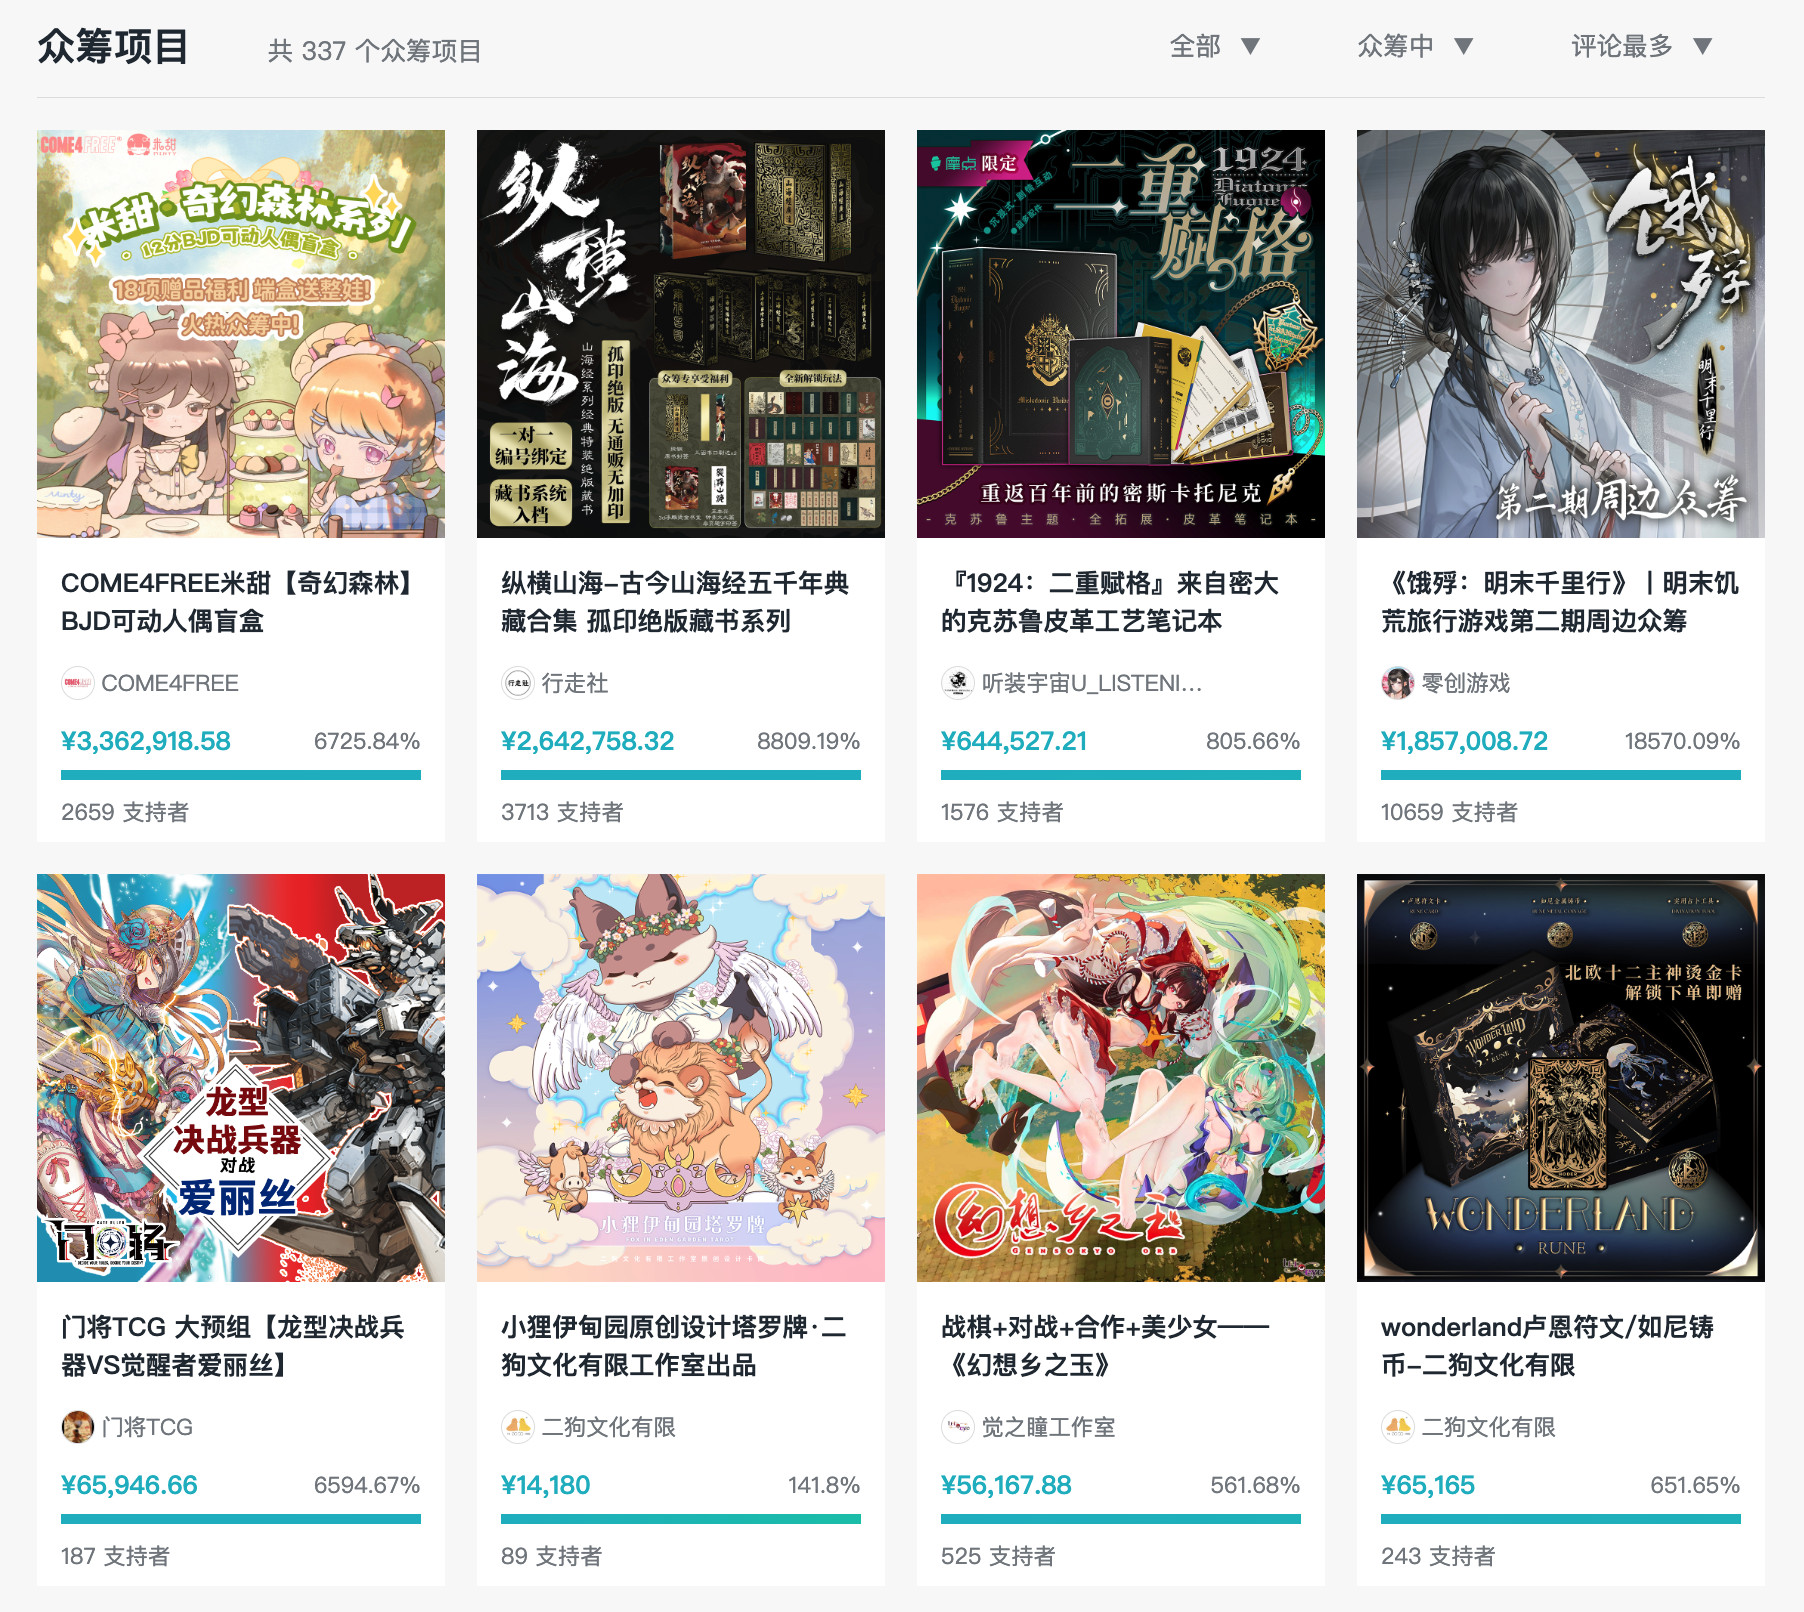
\includegraphics[width=0.75\linewidth]{modian_snapshots.jpg}
    \caption{A snapshot of campaign listings}
    \label{fig:Snapshot_listings}
\end{figure}

\begin{figure}[ht!]
    \centering
    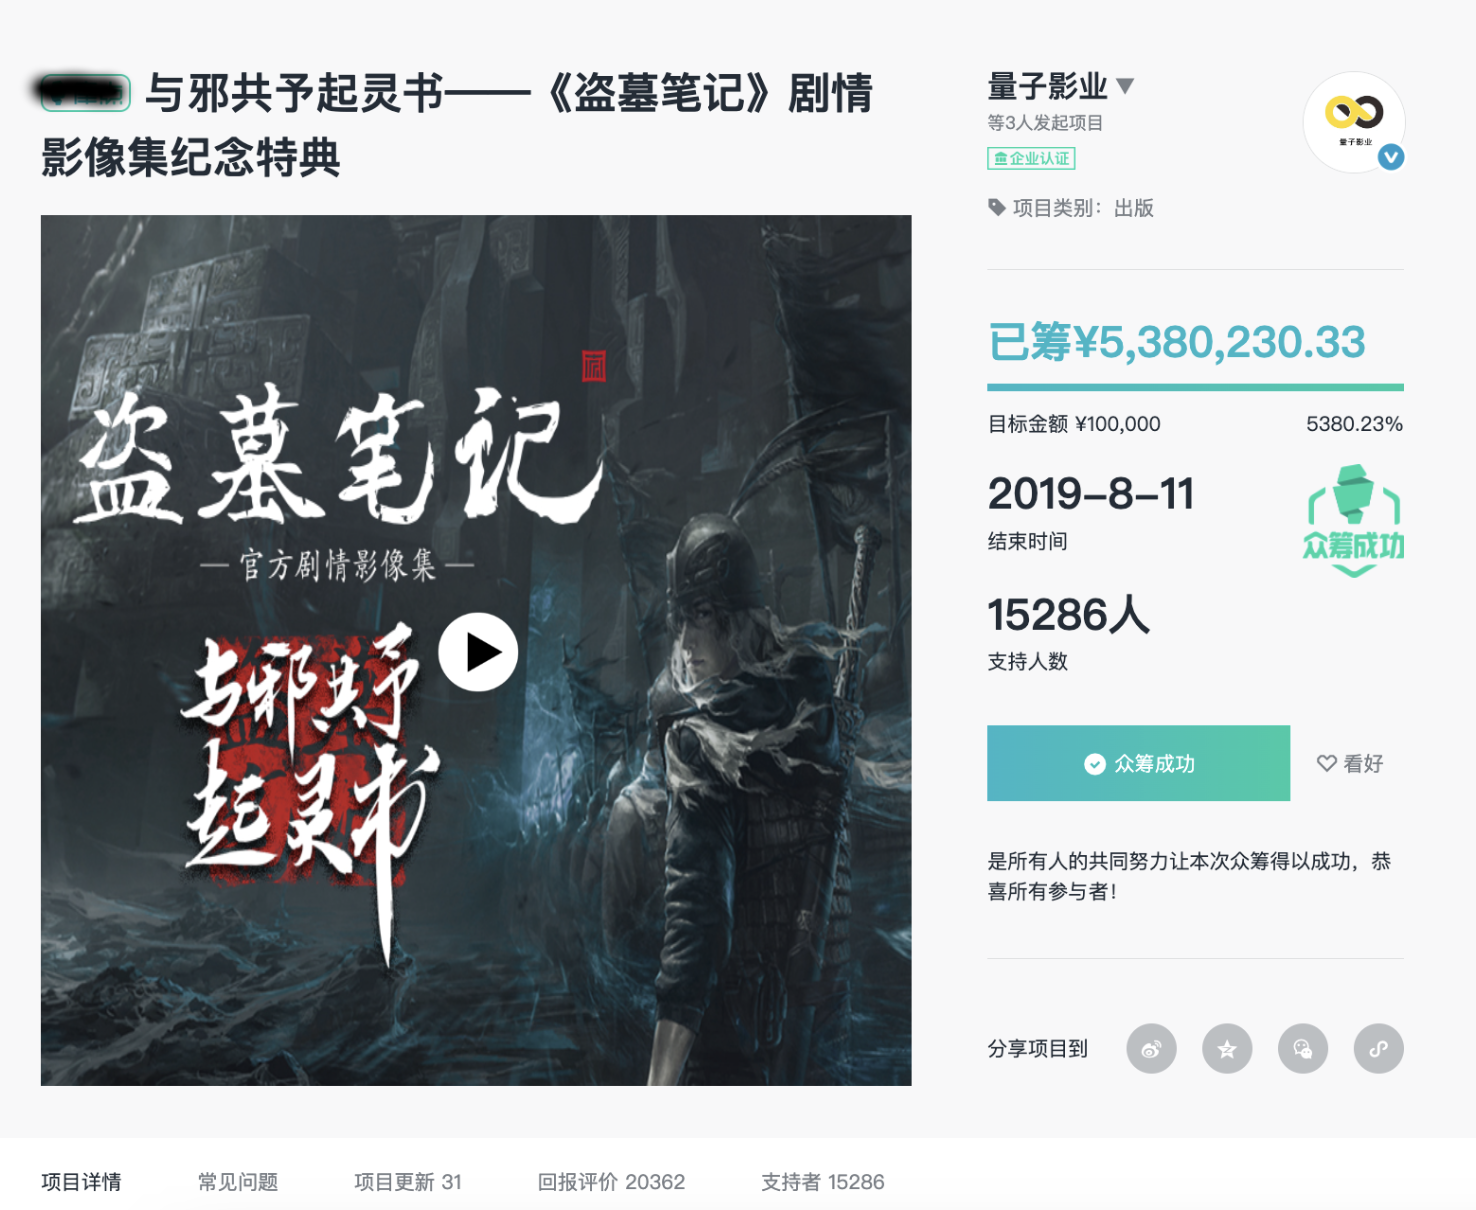
\includegraphics[width=0.75\linewidth]{modian_sample.png}
    \caption{A snapshot of the details of a campaign}
    \label{fig:Snapshot}
\end{figure}

To understand the mode of text positions, we first divide an image into nine blocks and number them from top to down and from left to right. For instance, the upper left one was numbered as 1, the upper center one was numbered as 2, etc. Blocks that are dominant by text were labeled as 1, while the others were labeled as 0. After that, the text positions of an image were coded based on the text labels of the blocks.  For instance, an image with blocks in the upper left (i.e., Position \emph{1}) and upper center (i.e., Position \emph{2}) were labeled as text dominant, then the text position mode of this image is encoded as \emph{1\_2}.  

When labeling the blocks of these images, we take the following procedures. First, we manually labeled the blocks of randomly selected 600 images, and each image was encoded independently by two research assistants. Around 85.0\% of the blocks were labeled consistently. For those blocks coded with different labels, they discuss to determine the final results. With these manually encoded labels, we then developed a machine learning model (i.e., CNN model) to predict the labels with the rest images. The accuracy of the CNN model is 72.8\% for the test data, indicating that the model is valid. 

As the results of the econometric analysis may suffer from the problem of endogeneity, we also conducted a series of experiments to cross-validate the findings. In Experiment (1), we generate ten groups of images by ChatGPT that could be used as cover images for some reward-based crowdfunding campaigns. Each group contains two similar images, with one image incorporated with text descriptions while the other does not. The participants were asked to compare the attractiveness of the images in each group and choose the one that that is more preferable. The order of the images in each group was randomized. A snapshot of this experiment is shown in Figure \ref{fig:Experiment1}. This experiment was designed to test Hypothesis 1. 



\begin{figure}[h!]
    \centering
    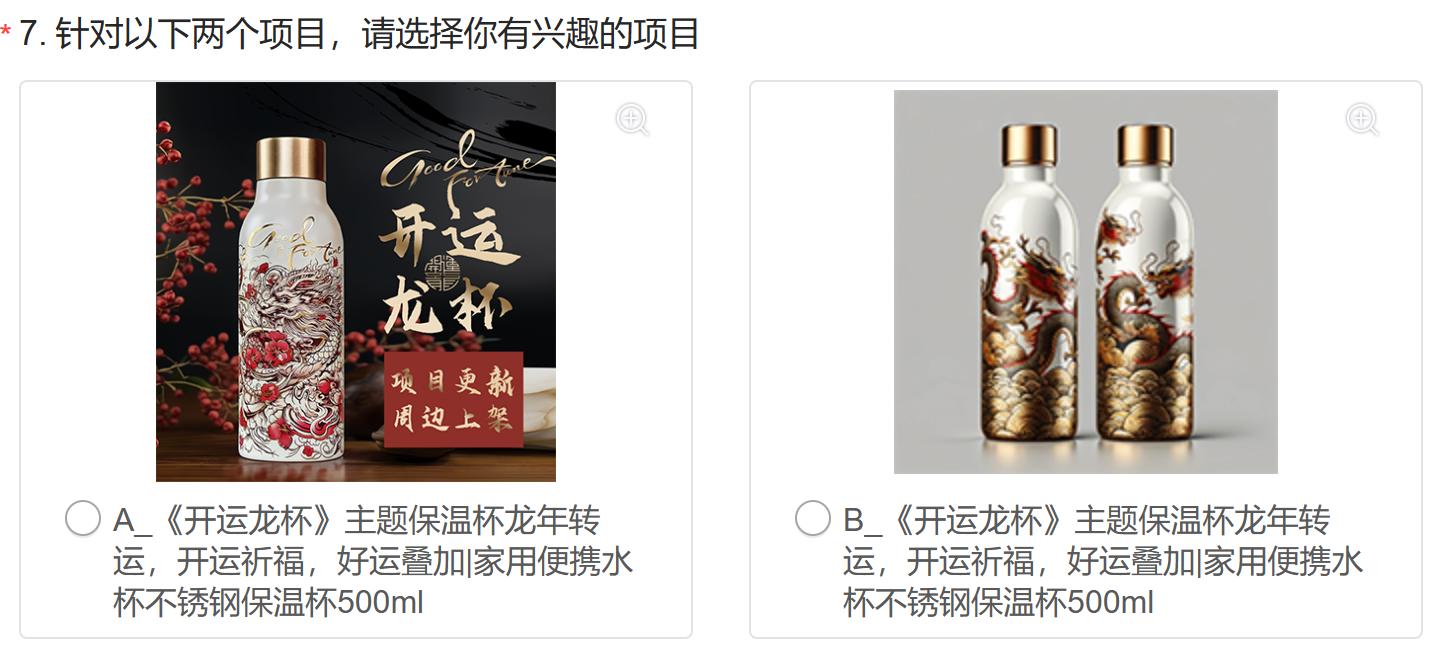
\includegraphics[width=0.8\linewidth]{experiment1.jpg}
    \caption{A snapshot of the Experiment (1).}
    \label{fig:Experiment1}
\end{figure}


\begin{figure}[h!]
    \centering
    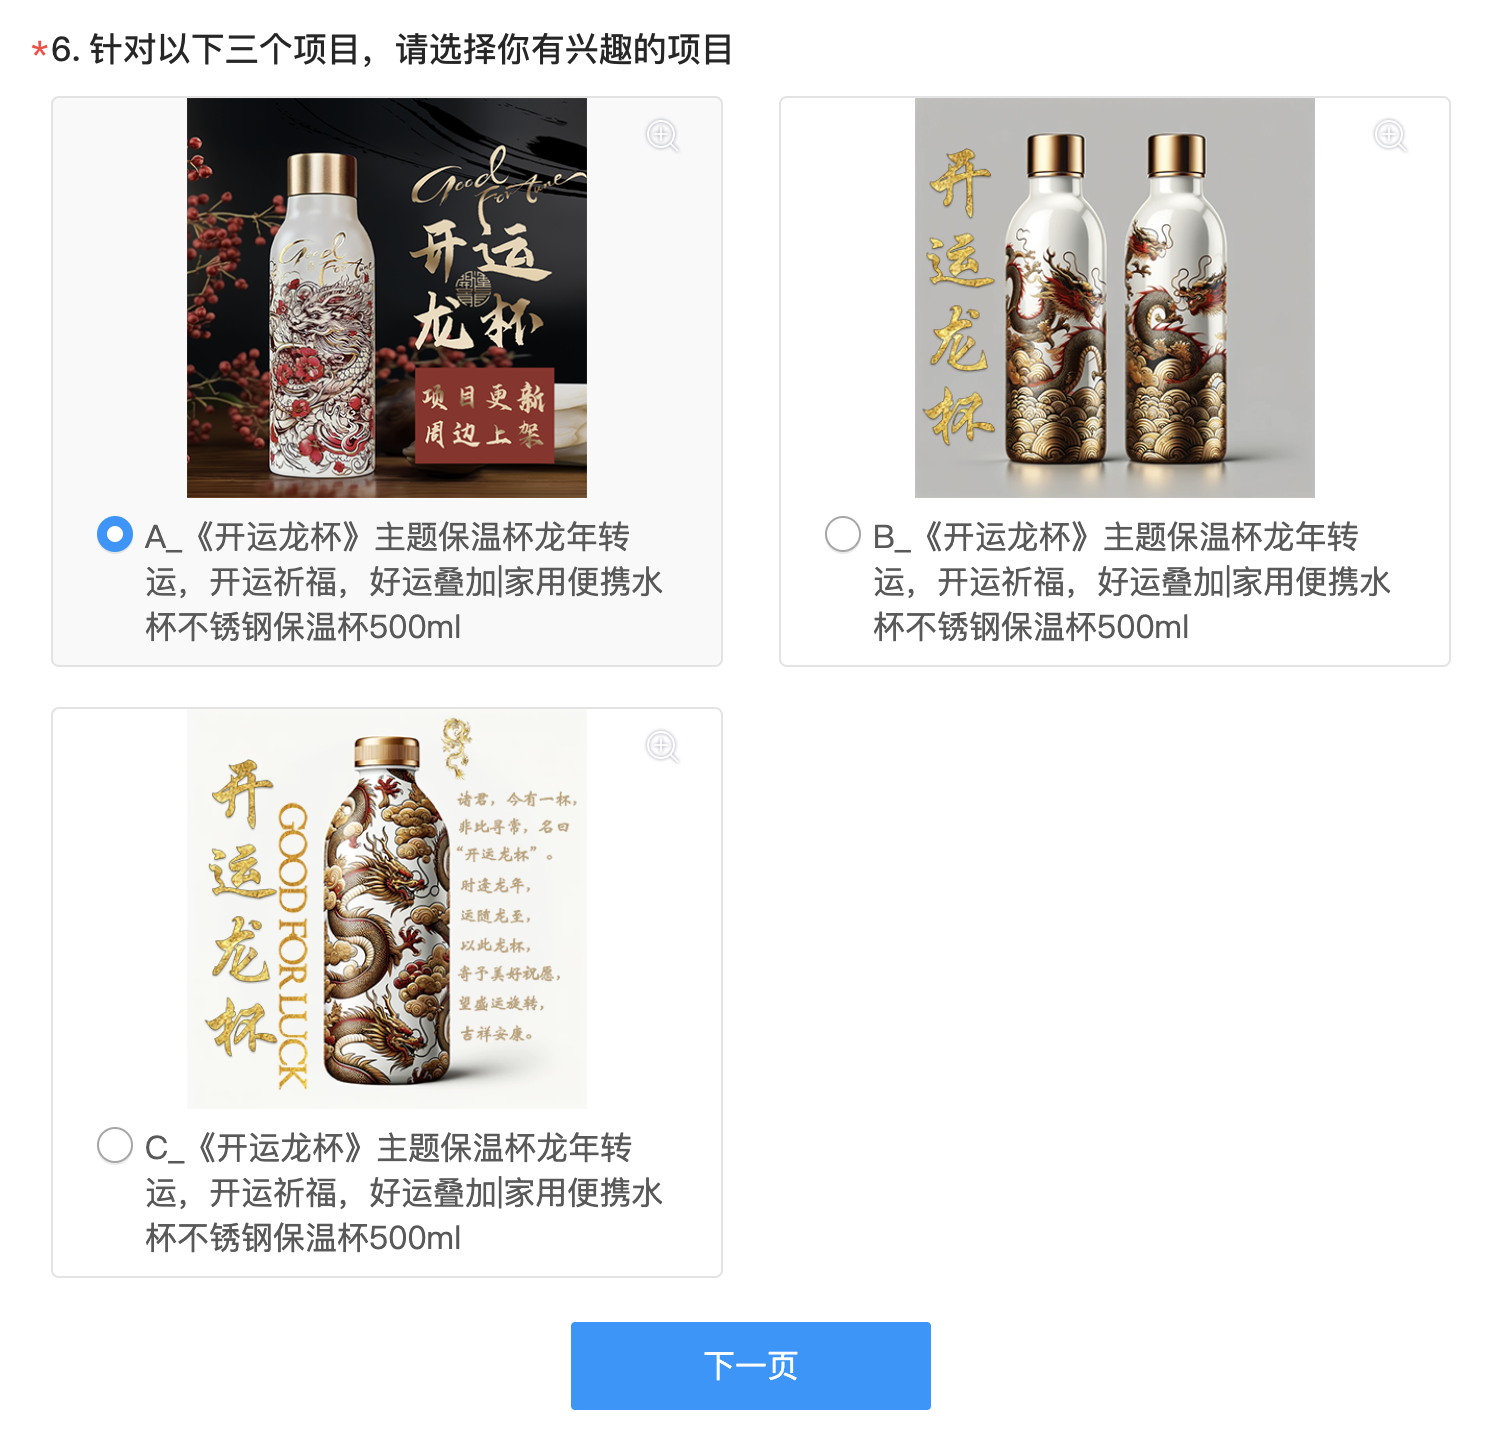
\includegraphics[width=0.8\linewidth]{experiment4.png}
    \caption{A snapshot of the Experiment (2).}
    \label{fig:Experiment4}
\end{figure}

In Experiment (2), we generate another ten groups of images by ChatGPT with each group containing three similar images. One image contains low-level density text, one contains median-level density text, and the rest one with high level of density. The participants were then asked to choose the most preferable image from these three images in each question. A snapshot of this experiment is shown in Figure \ref{fig:Experiment4}. This experiment was designed to test Hypothesis 2. 

As the size of text in an image could influence participants' perceptions, we designed another experiment that fixes the size of text and varies only the text density. In Experiment (3), we choose another ten groups of images by ChatGPT with each containing two similar images, one containing low-level density text, and the other with high-level density text. A snapshot of this experiment is shown in Figure \ref{fig:Experiment5}.

\begin{figure}[h!]
    \centering
    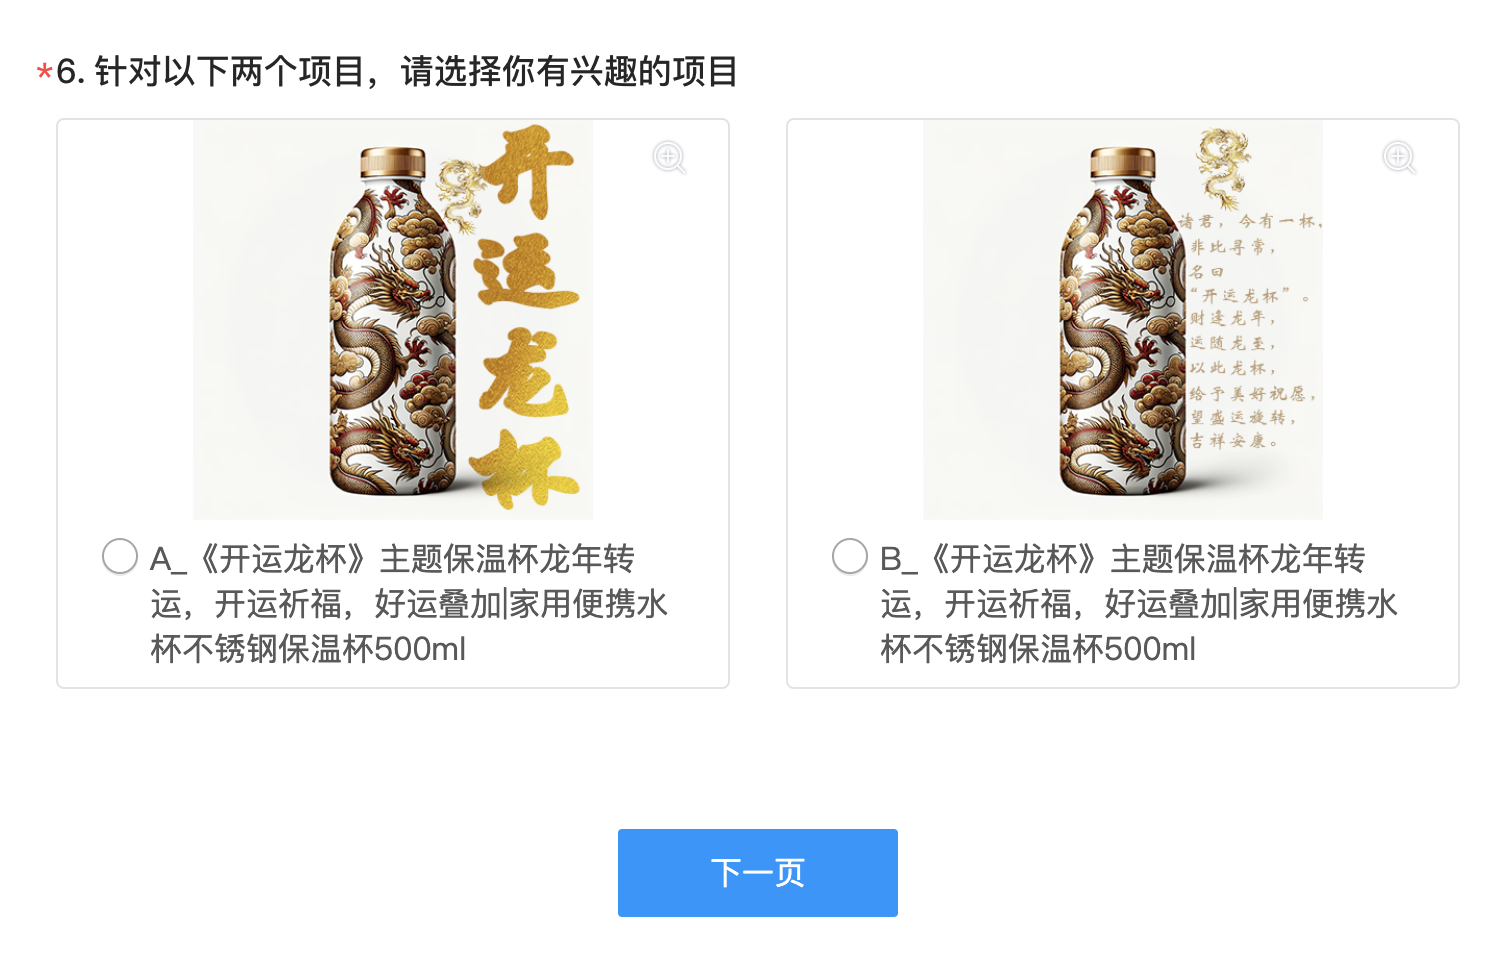
\includegraphics[width=0.8\linewidth]{experiment5.png}
    \caption{A snapshot of Experiment (3).}
    \label{fig:Experiment5}
\end{figure}

To test Hypothesis 3, we designed Experiment (4). In this experiment, we generated ten groups of images each containing two similar images, one with text in the center while the other not, participants were asked to choose the one that was preferable in each group. A snapshot of the experiment is shown in Figure \ref{fig:Experiment6}.

\begin{figure}[h!]
    \centering
    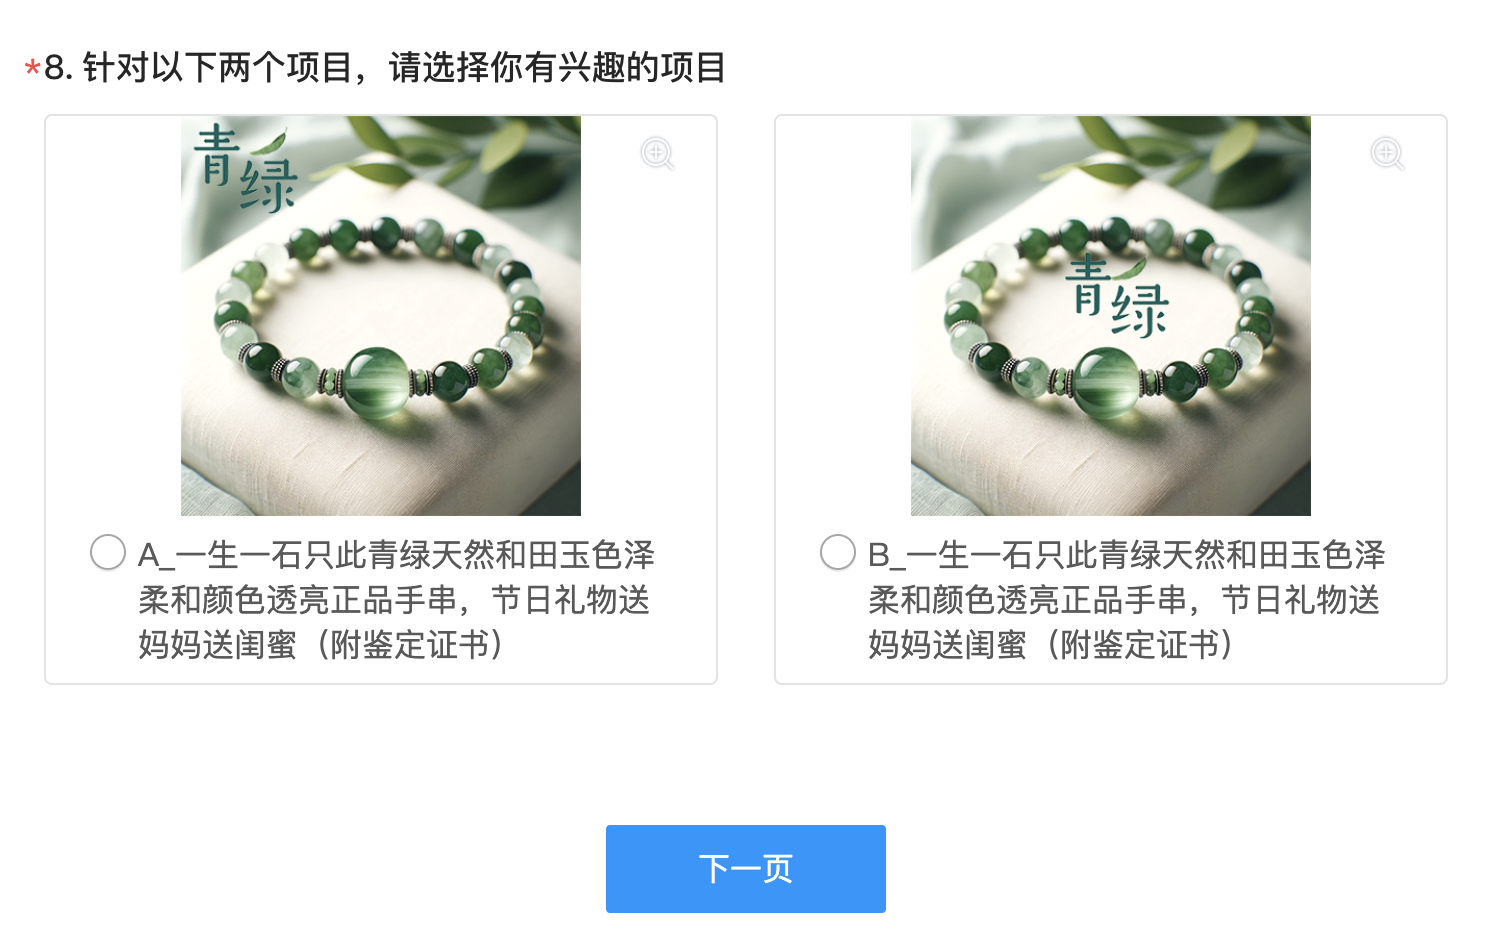
\includegraphics[width=0.8\linewidth]{experiment6.png}
    \caption{A snapshot of Experiment (4).}
    \label{fig:Experiment6}
\end{figure}



\subsection{Variables}
We investigate how text in images affects the attractiveness of reward-based campaigns. As the cover image is the most important image of a campaign, we only study the effect of the text in the cover image. Following the prior literature, we use the number of bids received in a campaign, \emph{BackerCount}, to measure campaign attractiveness. As $BackerCount$ is highly skewed, this variable is logarithmly transformed, $LogBackerCount = log(BackerCount+1)$.  The main independent variables are the text characteristics in the cover image of a campaign. We consider the following variables: $ContainText$, whether there are any texts in an image. $TextDentisy$, the text density calculated by dividing the number of text in the cover image by the size it occupied, this variable is also log-transformed in the regression analysis. $HorizonBlock$, the horizontal positions of the text in a cover image.  $VertBlock$, the vertical positions of the text in a cover image. 

While encoding $HorizonBlock$, we divide an image into three subsections based on horizontal positions, namely upper, middle, and bottom. Those images with text mode labeled as $1, 2, 3$ or any combinations were categorized as $Upper$, and those labeled as $4,5,6$ or any combinations were categorized as $Middle$, while those labeled as $7,8,9$ or any combinations were categorized as $Bottom$. Those who cannot be categorized into these three groups were discarded. The $Middle$ group was used as the reference group in the analysis.

While encoding $VertBlock$, we also divide an image into three subsections based on their vertical positions, namely left, center, and right. These images with text mode labeled as $1,4,7$ or any combinations were categorized as $Left$, and those labeled as $2,5,8$ or any combinations were labeled as $Center$, while those labeled as $3,6,9$ or any combinations were labeled as $Right$. Those who cannot be categorized into these groups were discarded. The $Center$ group was used as the reference group in the analysis. 

We incorporate various campaign-level control variables, including campaign features, image features, and textual features, into the model estimation.$Goal$, the goal money that needs to be raised for a campaign, $Launcher$, the number of launchers of a campaign, $Video$, the number of videos included in a campaign, $Face$, the number of facial images detected in a campaign, $Update$, the number of updates by launchers to the original campaign message, $Comment$, the number of comments posted by reviewers to a campaign, $Description$, the number of words in a description of a campaign, $Title$, the number of words in a title of a campaign. Following \parencite{zhao_multi-modal_2022}, we also incorporated the text features of campaign titles. $Readability$, the readability level of the title of a campaign. It is measured using Flesch reading ease score, $206.835 - (1.015 * ASL) - (84.6 * (Nsy / Nw))$, where ASL is the average sentence length in words, Nsy denotes the number of syllables, and Nw denotes WordCount. $Polarity$, the polarity score of the title of a campaign. It ranges from -1 to 1, with 1 being extremely positive, and -1 being extremely negative. $Subjectivity$, the subjectivity level of the title of a campaign. It ranges from 0 to 1, with 0 being extremely objective, and 1 extremely subjective. 

A list of variables is described in Table \ref{tab:Vairalbes}. 
\begin{table}
    \centering
    \caption{Summary of variables and their operationalization}
    \label{tab:Vairalbes}

    \begin{tabular}{lp{0.75\textwidth}}
    \\[-1.8ex]\hline 
\hline \\[-1.8ex] 
\bf Variables & \bf Operationalization \\
\hline \\[-1.8ex] 
Goal & The goal money that needs to be raised for a campaign \\
Launcher & The number of launchers of a campaign \\
Video         & The number of videos shown in a campaign\\
Image         & The number of images shown in a campaign\\
Face         & The number of facial images shown in a campaign \\
Update         & The number of updates to the original campaign message\\
Comment         & The number of comments toward a campaign\\
Description  &  The number of words in campaign description\\
Title & The number of words in campaign title \\
Readability & The readability level of campaign title (using TextStat) \\
Polarity & The polarity score of campaign title (using TextBlob) \\
Subjectivity & The subjectivity score of campaign title (using TextBlob) \\
BackerMoney & The total money backed by investors to the campaign \\
BackerCount & the total bids launched by investors to the campaign \\
ContainText & Whether text is incorporated in the cover image of a campaign. \\
TextDensity & The density of text in a cover image of a campaign, 
calculated by dividing text number by text area \\
\hline
    \hline \\[-1.8ex] 
    \end{tabular}
\end{table}

\subsection{Econometric models}
To test Hypothesis 1, we employ the following regression model:
\begin{equation}
    LogBackerCount = \alpha ContainText + \gamma Controls + \varepsilon
\end{equation}
where $ContainText$ indicates whether text is incorporated in the cover image of a campaign, $LogBackerCount$ is the log-transformed value of $BackerCount$. 

To test Hypothesis 2, we employ the following regression model:
\begin{equation}
    LogBackerCount = \alpha LogTextDensity + \beta LogTextDensity^2 + \gamma Controls + \varepsilon 
\end{equation}

where $LogTextDensity$ indicates the density of text, this variable is log-transformed as $TextDensity$ is highly skewed.

To test Hypothesis 3, we use the following regression model:
\begin{equation}
    LogBackerCount = \alpha HorizonBlock +\beta VertBlock +  \gamma Controls + \varepsilon 
\end{equation}
where $HorizonBlock$ indicates the horizontal positions of the text incorporated in the cover image, while the $VertBlock$ indicates the vertical positions of the text in the cover image. For $HorizonBlock$, there are three groups, namely $Upper$, $Middle$, and $Lower$, with $Middle$ as the reference group; while for $VertBlock$, there are three groups, namely $Left$, $Center$, and $Right$, with $Center$ as the reference group. 

\subsection{Data Description}
Here are the summaries of the main variables used in this paper. A description analysis of the variables are shown in Table \ref{tab: Data Description}.
\begin{table}
  \caption{Descriptive analysis} 
  \label{tab: Data Description} 
% \begin{tabular}{@{\extracolsep{5pt}}lccccc}
\begin{tabular}{lccccc}
\\[-1.8ex]\hline 
\hline \\[-1.8ex] 
Statistic & \multicolumn{1}{c}{N} & \multicolumn{1}{c}{Mean} & \multicolumn{1}{c}{St. Dev.} & \multicolumn{1}{c}{Min} & \multicolumn{1}{c}{Max} \\ 
\hline \\[-1.8ex] 
BackerCount & 10,055 & 364.145 & 1,683.617 & 0 & 87,674 \\ 
BackerMoney & 10,055 & 102,127.200 & 443,968.000 & 0.000 & 20,202,405.000 \\ 
ContainText & 10,055 & 0.929 & 0.256 & 0 & 1 \\ 
Goal & 10,055 & 25,647.830 & 60,388.810 & 1 & 1,500,000 \\ 
Video & 10,055 & 0.211 & 1.140 & 0 & 41 \\ 
Image & 10,055 & 17.579 & 14.016 & 0 & 264 \\ 
Face & 10,055 & 0.122 & 0.391 & 0 & 8 \\ 
Update & 10,055 & 7.988 & 9.498 & 0 & 115 \\ 
Comment & 10,055 & 337.621 & 1,716.182 & 0 & 89,010 \\ 
Description & 10,055 & 262.027 & 845.447 & 0 & 10,883 \\ 
Title & 10,055 & 21.402 & 4.742 & 3 & 44 \\ 
Readability & 10,055 & 55.624 & 24.776 & $-$132.590 & 206.840 \\ 
Polarity & 10,055 & 0.114 & 0.259 & $-$1.000 & 1.000 \\ 
Subjectivity & 10,055 & 0.396 & 0.300 & 0.000 & 1.000 \\ 
\hline \\[-1.8ex] 
\end{tabular} 
\end{table} 


\section{Results}
\subsection{Econometric analysis}
% Table created by stargazer v.5.2.3 by Marek Hlavac, Social Policy Institute. E-mail: marek.hlavac at gmail.com
% Date and time: Tue, Apr 30, 2024 - 03:57:49 PM

Some variables are highly skewed, so these variables are log-transformed before they were used in the regression analysis. The density distributions the main variable $LogBackerCount$ versus $ContainText$ is shown in the left of Figure \ref{fig:Description}. While the relationship between $LogBackerCount$ and $LogTextDensity$ is shown in the right of Figure \ref{fig:Description}.
\begin{figure}
    \centering
    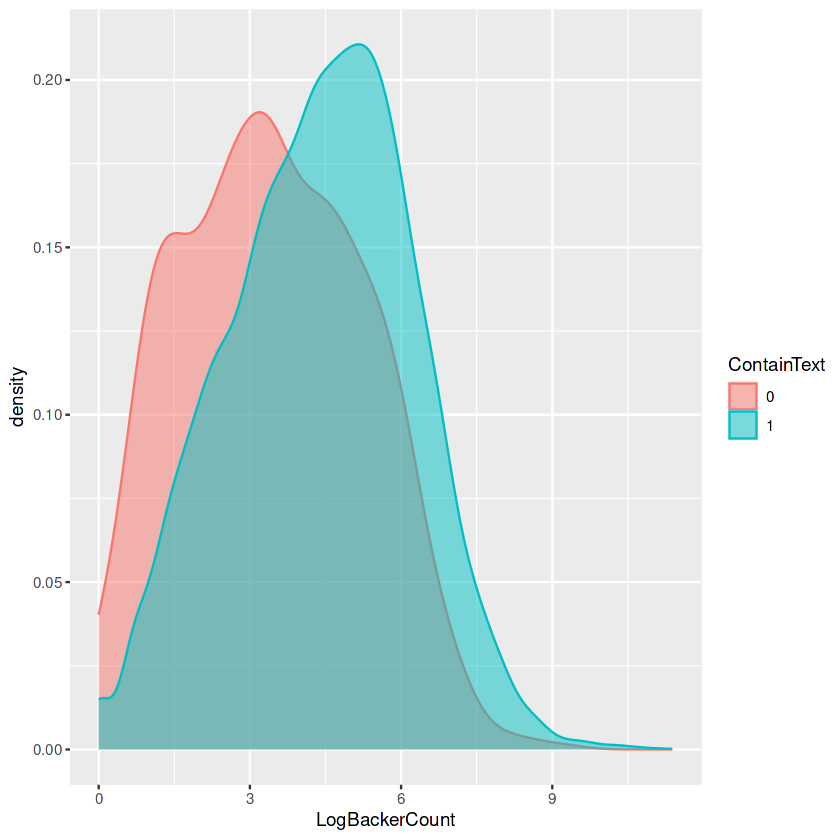
\includegraphics[width=0.4\linewidth]{Density.png}
    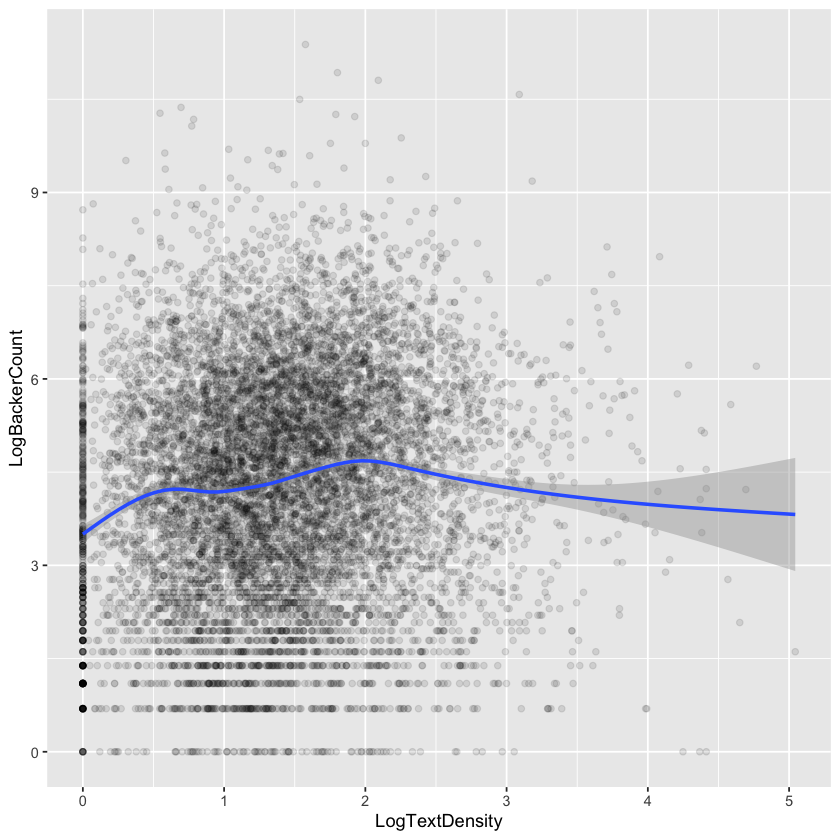
\includegraphics[width=0.4\linewidth]{TextDensity.png}
    \caption{The relationship between main variables and \textit{LogBackerCount}}
    \label{fig:Description}
\end{figure}


% Table created by stargazer v.5.2.3 by Marek Hlavac, Social Policy Institute. E-mail: marek.hlavac at gmail.com
% Date and time: Wed, May 15, 2024 - 18:51:50
% Requires LaTeX packages: dcolumn 
\begin{table}[!htbp] \centering 
    \caption{The impact of text in cover image on campaign attractiveness} 
    \label{} 
\resizebox{1\linewidth}{!}{
  \begin{tabular}{@{\extracolsep{1pt}}lD{.}{.}{-3} D{.}{.}{-3} D{.}{.}{-3} D{.}{.}{-3} D{.}{.}{-3} D{.}{.}{-3} } 
  \\[-1.8ex]\hline 
  \hline \\[-1.8ex] 
   & \multicolumn{6}{c}{\textit{Dependent variable:}} \\ 
  \cline{2-7} 
  \\[-1.8ex] & \multicolumn{6}{c}{LogBackerCount} \\ 
  \\[-1.8ex] & \multicolumn{1}{c}{(1)} & \multicolumn{1}{c}{(2)} & \multicolumn{1}{c}{(3)} & \multicolumn{1}{c}{(4)} & \multicolumn{1}{c}{(5)} & \multicolumn{1}{c}{(6)}\\ 
  \hline \\[-1.8ex] 
   ContainText &  & 0.517^{***} &  &  &  &  \\ 
    &  & (0.052) &  &  &  &  \\ 
    LogTextDensity &  &  & 0.104^{***} & 0.424^{***} &  &  \\ 
    &  &  & (0.018) & (0.054) &  &  \\ 
    LogTextDensity2 &  &  &  & -0.103^{***} &  &  \\ 
    &  &  &  & (0.016) &  &  \\ 
    HorizonBlockBottom &  &  &  &  & 0.052 &  \\ 
    &  &  &  &  & (0.108) &  \\ 
    HorizonBlockUpper &  &  &  &  & -0.128 &  \\ 
    &  &  &  &  & (0.096) &  \\ 
    VertBlockLeft &  &  &  &  &  & -0.195^{**} \\ 
    &  &  &  &  &  & (0.096) \\ 
    VertBlockRight &  &  &  &  &  & -0.279^{***} \\ 
    &  &  &  &  &  & (0.098) \\ 
    LogGoal & 0.199^{***} & 0.193^{***} & 0.194^{***} & 0.191^{***} & 0.221^{***} & 0.170^{***} \\ 
    & (0.011) & (0.011) & (0.011) & (0.011) & (0.028) & (0.034) \\ 
    Video & -0.074^{***} & -0.067^{***} & -0.070^{***} & -0.068^{***} & -0.111^{***} & -0.024 \\ 
    & (0.012) & (0.012) & (0.012) & (0.012) & (0.028) & (0.026) \\ 
    Image & 0.007^{***} & 0.007^{***} & 0.007^{***} & 0.006^{***} & 0.006^{**} & 0.003 \\ 
    & (0.001) & (0.001) & (0.001) & (0.001) & (0.003) & (0.003) \\ 
    Face & -0.041 & -0.039 & -0.039 & -0.032 & -0.109 & 0.152 \\ 
    & (0.034) & (0.034) & (0.034) & (0.034) & (0.089) & (0.114) \\ 
    Update & 0.068^{***} & 0.068^{***} & 0.067^{***} & 0.067^{***} & 0.073^{***} & 0.065^{***} \\ 
    & (0.002) & (0.002) & (0.002) & (0.002) & (0.004) & (0.005) \\ 
    LogComment & 0.250^{***} & 0.246^{***} & 0.249^{***} & 0.248^{***} & 0.232^{***} & 0.325^{***} \\ 
    & (0.007) & (0.007) & (0.007) & (0.007) & (0.017) & (0.022) \\ 
    LogDescription & -0.003 & -0.001 & -0.0003 & 0.004 & 0.016 & 0.026^{*} \\ 
    & (0.005) & (0.005) & (0.005) & (0.005) & (0.014) & (0.015) \\ 
    Title & 0.038^{***} & 0.037^{***} & 0.037^{***} & 0.036^{***} & 0.027^{***} & 0.024^{***} \\ 
    & (0.003) & (0.003) & (0.003) & (0.003) & (0.008) & (0.009) \\ 
    Readability & -0.001 & -0.001 & -0.0004 & -0.0003 & -0.004^{***} & 0.0001 \\ 
    & (0.001) & (0.001) & (0.001) & (0.001) & (0.001) & (0.002) \\ 
    Polarity & -0.299^{***} & -0.304^{***} & -0.313^{***} & -0.322^{***} & -0.498^{***} & -0.070 \\ 
    & (0.058) & (0.058) & (0.058) & (0.058) & (0.153) & (0.181) \\ 
    Subjectivity & -0.154^{***} & -0.150^{***} & -0.137^{***} & -0.132^{***} & -0.222^{*} & -0.041 \\ 
    & (0.050) & (0.050) & (0.050) & (0.050) & (0.130) & (0.148) \\ 
    Constant & 0.269^{**} & -0.129 & 0.173 & 0.025 & 0.525^{*} & 0.436 \\ 
    & (0.110) & (0.117) & (0.111) & (0.114) & (0.307) & (0.335) \\ 
   \hline \\[-1.8ex] 
  Observations & \multicolumn{1}{c}{10,055} & \multicolumn{1}{c}{10,055} & \multicolumn{1}{c}{10,055} & \multicolumn{1}{c}{10,055} & \multicolumn{1}{c}{1,504} & \multicolumn{1}{c}{950} \\ 
  R$^{2}$ & \multicolumn{1}{c}{0.472} & \multicolumn{1}{c}{0.477} & \multicolumn{1}{c}{0.474} & \multicolumn{1}{c}{0.476} & \multicolumn{1}{c}{0.483} & \multicolumn{1}{c}{0.564} \\ 
  \hline 
  \hline \\[-1.8ex] 
  \textit{Note:}  & \multicolumn{6}{l}{$^{*}$p$<$0.1; $^{**}$p$<$0.05; $^{***}$p$<$0.01} \\ 
  \end{tabular} 
  }
  \end{table}
  
% Table created by stargazer v.5.2.3 by Marek Hlavac, Social Policy Institute. E-mail: marek.hlavac at gmail.com
% Date and time: Tue, Apr 30, 2024 - 03:58:36 PM
% Requires LaTeX packages: dcolumn 
\begin{table} \centering 
  \caption{The impact of text inclusion in the cover image on campaign attractiveness} 
  \label{tab: Text Inclusion} 
% \begin{tabular}{@{\extracolsep{5pt}}lD{.}{.}{-3} D{.}{.}{-3} D{.}{.}{-3} D{.}{.}{-3} } 
\begin{tabular}{lD{.}{.}{-3} D{.}{.}{-3} D{.}{.}{-3} D{.}{.}{-3} } 
\\[-1.8ex]\hline 
\hline \\[-1.8ex] 
\\[-1.8ex] & \multicolumn{2}{c}{LogBackerMoney} & \multicolumn{2}{c}{LogBackerCount} \\ 
\\[-1.8ex] & \multicolumn{1}{c}{(1)} & \multicolumn{1}{c}{(2)} & \multicolumn{1}{c}{(3)} & \multicolumn{1}{c}{(4)}\\ 
\hline \\[-1.8ex] 
 ContainText &  & 0.457^{***} &  & 0.517^{***} \\ 
  &  & (0.071) &  & (0.052) \\ 
  LogGoal & 0.435^{***} & 0.430^{***} & 0.199^{***} & 0.193^{***} \\ 
  & (0.015) & (0.015) & (0.011) & (0.011) \\ 
  Video & 0.002 & 0.008 & -0.074^{***} & -0.067^{***} \\ 
  & (0.016) & (0.016) & (0.012) & (0.012) \\ 
  Image & 0.017^{***} & 0.016^{***} & 0.007^{***} & 0.007^{***} \\ 
  & (0.001) & (0.001) & (0.001) & (0.001) \\ 
  Face & -0.037 & -0.035 & -0.041 & -0.039 \\ 
  & (0.046) & (0.046) & (0.034) & (0.034) \\ 
  Update & 0.092^{***} & 0.092^{***} & 0.068^{***} & 0.068^{***} \\ 
  & (0.002) & (0.002) & (0.002) & (0.002) \\ 
  LogComment & 0.169^{***} & 0.166^{***} & 0.250^{***} & 0.246^{***} \\ 
  & (0.009) & (0.009) & (0.007) & (0.007) \\ 
  LogDescription & -0.041^{***} & -0.039^{***} & -0.003 & -0.001 \\ v
  & (0.007) & (0.007) & (0.005) & (0.005) \\ 
  Title & 0.036^{***} & 0.035^{***} & 0.038^{***} & 0.037^{***} \\ 
  & (0.004) & (0.004) & (0.003) & (0.003) \\ 
  Readability & 0.000 & 0.000 & -0.001 & -0.001 \\ 
  & (0.001) & (0.001) & (0.001) & (0.001) \\ 
  Polarity & -0.128 & -0.133^{*} & -0.299^{***} & -0.304^{***} \\ 
  & (0.079) & (0.079) & (0.058) & (0.058) \\ 
  Subjectivity & -0.195^{***} & -0.192^{***} & -0.154^{***} & -0.150^{***} \\ 
  & (0.069) & (0.068) & (0.050) & (0.050) \\ 
  Constant & 3.302^{***} & 2.950^{***} & 0.269^{**} & -0.129 \\ 
  & (0.151) & (0.160) & (0.110) & (0.117) \\ 
  \hline
 Observations & \multicolumn{1}{c}{10,055} & \multicolumn{1}{c}{10,055} & \multicolumn{1}{c}{10,055} & \multicolumn{1}{c}{10,055} \\ 
R$^{2}$ & \multicolumn{1}{c}{0.414} & \multicolumn{1}{c}{0.416} & \multicolumn{1}{c}{0.472} & \multicolumn{1}{c}{0.477} \\ 
\hline \\[-1.8ex] 
\textit{Notes:} & \multicolumn{4}{l}{$^{***}$Significant at the 1 percent level.} \\ 
 & \multicolumn{4}{l}{$^{**}$Significant at the 5 percent level.} \\ 
 & \multicolumn{4}{l}{$^{*}$Significant at the 10 percent level.} \\ 
\end{tabular} 
\end{table} 

The results in \ref{tab: Text Inclusion} show that $ContainText$ has a significant impact on the dependent variable of $LogBackerCount$, suggesting that incorporating text in the cover image could significantly improve the attractiveness of a campaign. Hypothesis 1 is supported.  

Then we examine the impact of text density in the cover image on campaign attractiveness. The results are shown in Table \ref{tab: Text U Shape}. The results show that the coefficient of the term $LogTextDensity$ is significant and positive, but the term $LogTextDensity2$ is negative, indicating that the relationship between text density and backer count is in an inverse U shape. Hypothesis 2 is supported.

\begin{table}\centering 
  \caption{The impact of text density in cover image on campaign attractiveness} 
  \label{tab: Text U Shape} 
\begin{tabular}{@{\extracolsep{1pt}}lD{.}{.}{-3} D{.}{.}{-3} D{.}{.}{-3} D{.}{.}{-3} } 
\\[-1.8ex]\hline 
\hline \\[-1.8ex] 
\\[-1.8ex] & \multicolumn{2}{c}{LogBackerMoney} & \multicolumn{2}{c}{LogBackerCount} \\ 
\\[-1.8ex] & \multicolumn{1}{c}{(1)} & \multicolumn{1}{c}{(2)} & \multicolumn{1}{c}{(3)} & \multicolumn{1}{c}{(4)}\\ 
\hline \\[-1.8ex] 
  LogTextDensity & 0.216^{***} & 0.800^{***} & 0.109^{***} & 0.312^{***} \\ 
  & (0.027) & (0.086) & (0.020) & (0.063) \\ 
  LogTextDensity2 &  & -0.186^{***} &  & -0.065^{***} \\ 
  &  & (0.026) &  & (0.019) \\ 
  Video & -0.011 & -0.013 & -0.060^{***} & -0.060^{***} \\ 
  & (0.018) & (0.018) & (0.013) & (0.013) \\ 
  Image & 0.017^{***} & 0.017^{***} & 0.007^{***} & 0.007^{***} \\ 
  & (0.001) & (0.001) & (0.001) & (0.001) \\ 
  Face & 0.003 & 0.013 & -0.015 & -0.012 \\ 
  & (0.050) & (0.049) & (0.036) & (0.036) \\ 
  Update & 0.098^{***} & 0.098^{***} & 0.071^{***} & 0.071^{***} \\ 
  & (0.002) & (0.002) & (0.002) & (0.002) \\ 
  LogComment & 0.237^{***} & 0.235^{***} & 0.274^{***} & 0.274^{***} \\ 
  & (0.009) & (0.009) & (0.007) & (0.007) \\ 
  LogDescription & -0.031^{***} & -0.024^{***} & 0.003 & 0.005 \\ 
  & (0.008) & (0.008) & (0.006) & (0.006) \\ 
  Title & 0.050^{***} & 0.049^{***} & 0.045^{***} & 0.044^{***} \\ 
  & (0.004) & (0.004) & (0.003) & (0.003) \\ 
  Readability & 0.001 & 0.001 & -0.000 & -0.000 \\ 
  & (0.001) & (0.001) & (0.001) & (0.001) \\ 
  Polarity & -0.174^{**} & -0.191^{**} & -0.301^{***} & -0.307^{***} \\ 
  & (0.083) & (0.083) & (0.060) & (0.060) \\ 
  Subjectivity & -0.110 & -0.102 & -0.115^{**} & -0.112^{**} \\ 
  & (0.072) & (0.072) & (0.052) & (0.052) \\ 
  Constant & 6.348^{***} & 6.009^{***} & 1.671^{***} & 1.554^{***} \\ 
  & (0.111) & (0.120) & (0.081) & (0.088) \\ 
 Observations & \multicolumn{1}{c}{9,344} & \multicolumn{1}{c}{9,344} & \multicolumn{1}{c}{9,344} & \multicolumn{1}{c}{9,344} \\ 
R$^{2}$ & \multicolumn{1}{c}{0.376} & \multicolumn{1}{c}{0.379} & \multicolumn{1}{c}{0.452} & \multicolumn{1}{c}{0.453} \\ 
\hline \\[-1.8ex] 
\textit{Notes:} & \multicolumn{4}{l}{$^{***}$Significant at the 1 percent level.} \\ 
 & \multicolumn{4}{l}{$^{**}$Significant at the 5 percent level.} \\ 
 & \multicolumn{4}{l}{$^{*}$Significant at the 10 percent level.} \\ 
\end{tabular} 
\end{table} 

Finally, we examine the impact of text position on campaign attractiveness. The results are shown in Table \ref{tab: Text Position}. Regarding the dependent variable $LogBackerCount$, it is shown that text in the $Upper$ blocks are less attractive than those in the $Middle$, and those text in the $Left$ and $Right$ are less attractive than those in the $Center$. 

% Table created by stargazer v.5.2.3 by Marek Hlavac, Social Policy Institute. E-mail: marek.hlavac at gmail.com
% Date and time: Thu, May 16, 2024 - 06:38:49 AM
% Requires LaTeX packages: dcolumn 
\begin{table}[!htbp] \centering 
  \caption{The impact of text alignment in cover image on campaign attractiveness} 
  \label{} 
\begin{tabular}{@{\extracolsep{5pt}}lD{.}{.}{-3} D{.}{.}{-3} D{.}{.}{-3} D{.}{.}{-3} } 
\\[-1.8ex]\hline 
\hline \\[-1.8ex] 
\\[-1.8ex] & \multicolumn{2}{c}{LogBackerMoney} & \multicolumn{2}{c}{LogBackerCount} \\ 
\\[-1.8ex] & \multicolumn{1}{c}{(1)} & \multicolumn{1}{c}{(2)} & \multicolumn{1}{c}{(3)} & \multicolumn{1}{c}{(4)}\\ 
\hline \\[-1.8ex] 
 HorizonBlockBottom & 0.195 &  & 0.052 &  \\ 
  & (0.157) &  & (0.108) &  \\ 
  HorizonBlockUpper & 0.051 &  & -0.128 &  \\ 
  & (0.140) &  & (0.096) &  \\ 
  VertBlockLeft &  & 0.257^{*} &  & -0.195^{**} \\ 
  &  & (0.136) &  & (0.096) \\ 
  VertBlockRight &  & 0.020 &  & -0.279^{***} \\ 
  &  & (0.140) &  & (0.098) \\ 
  LogGoal & 0.398^{***} & 0.428^{***} & 0.221^{***} & 0.170^{***} \\ 
  & (0.041) & (0.049) & (0.028) & (0.034) \\ 
  Video & -0.070^{*} & 0.094^{**} & -0.111^{***} & -0.024 \\ 
  & (0.040) & (0.038) & (0.028) & (0.026) \\ 
  Image & 0.018^{***} & 0.012^{***} & 0.006^{**} & 0.003 \\ 
  & (0.004) & (0.004) & (0.003) & (0.003) \\ 
  Face & -0.067 & 0.139 & -0.109 & 0.152 \\ 
  & (0.129) & (0.163) & (0.089) & (0.114) \\ 
  Update & 0.101^{***} & 0.091^{***} & 0.073^{***} & 0.065^{***} \\ 
  & (0.006) & (0.007) & (0.004) & (0.005) \\ 
  LogComment & 0.154^{***} & 0.182^{***} & 0.232^{***} & 0.325^{***} \\ 
  & (0.025) & (0.031) & (0.017) & (0.022) \\ 
  LogDescription & -0.040^{*} & 0.007 & 0.016 & 0.026^{*} \\ 
  & (0.021) & (0.021) & (0.014) & (0.015) \\ 
  Title & 0.045^{***} & 0.028^{**} & 0.027^{***} & 0.024^{***} \\ 
  & (0.011) & (0.013) & (0.008) & (0.009) \\ 
  Readability & -0.002 & 0.002 & -0.004^{***} & 0.000 \\ 
  & (0.002) & (0.002) & (0.001) & (0.002) \\ 
  Polarity & -0.564^{**} & 0.271 & -0.498^{***} & -0.070 \\ 
  & (0.222) & (0.258) & (0.153) & (0.181) \\ 
  Subjectivity & -0.235 & -0.227 & -0.222^{*} & -0.041 \\ 
  & (0.189) & (0.211) & (0.130) & (0.148) \\ 
  Constant & 3.394^{***} & 3.262^{***} & 0.525^{*} & 0.436 \\ 
  & (0.446) & (0.477) & (0.307) & (0.335) \\ 
 Observations & \multicolumn{1}{c}{1,504} & \multicolumn{1}{c}{950} & \multicolumn{1}{c}{1,504} & \multicolumn{1}{c}{950} \\ 
R$^{2}$ & \multicolumn{1}{c}{0.386} & \multicolumn{1}{c}{0.441} & \multicolumn{1}{c}{0.483} & \multicolumn{1}{c}{0.564} \\ 
\hline \\[-1.8ex] 
\textit{Notes:} & \multicolumn{4}{l}{*p$<$0.1, **p$<$0.05, ***p$<$0.01} \\ 
\end{tabular}  

Notes: The reference group in (1) and (3) is $Middle$; while the reference group in (2) and (4) is $Center$. 
\end{table} 


\subsection{Experiments}
Whether launchers incorporate text in the cover image may be influenced by the campaign characteristics, and some of them may be unobservant. Thus the results may suffer from the problem of endogeneity. To tackle this problem, we designed a series of experiments. The details of the experiments are described in previous sections. 

\subsubsection{Experiment (1)}
The results of Experiment (1) show that images with text incorporated are preferable. A total of 45 participants attended this experiment, with 23 males and 22 females. The distributions of the responses for the preferences of the images are shown in Table \ref{tab:Experiment1}. The Chi-square value is 74.9, p<0.01, indicating that images with text are significantly preferable.  


\begin{table}
    \centering
\caption{Frequency of responses of Experiment (1)}
\label{tab:Experiment1}
    \begin{tabular}{ccc} 
    \hline \\[-1.8ex] 
 \textbf{Item}& \textbf{With Text}&\textbf{Without Text}\\ 
 \hline \\[-1.8ex]
         \textbf{Group1}&  39& 6\\ 
         \textbf{Group2}&  34& 11\\ 
         \textbf{Group3}&  25& 20\\ 
         \textbf{Group4}&  20& 25\\ 
         \textbf{Group5}&  27& 18\\ 
         \textbf{Group6}&  20& 25\\ 
         \textbf{Group7}&  31& 14\\ 
         \textbf{Group8}&  28& 17\\ 
         \textbf{Group9}&  7& 38\\ 
         \textbf{Group10}&  37& 8\\ 
         \hline \\ [-1.8ex] 
    \end{tabular}  
\end{table}

A summary of the frequencies of responses of Experiment (1) is shown in Figure \ref{fig:DistExperiment3}.

\begin{figure}
    \centering
    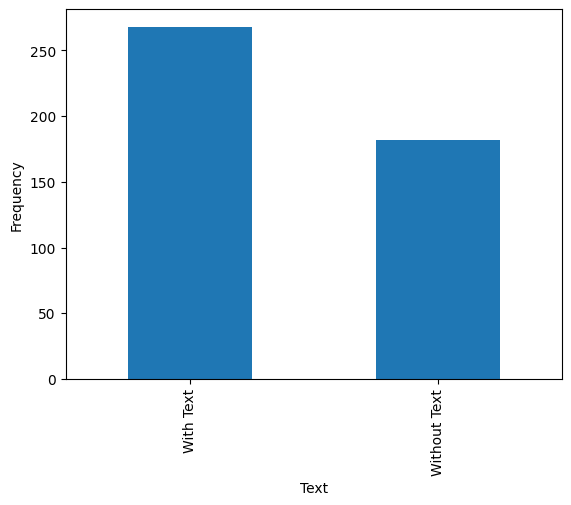
\includegraphics[width=0.75\linewidth]{distexperiment3.png}
    \caption{Distribution of responses of Experiment (1)}
    \label{fig:DistExperiment3}
\end{figure}

\subsubsection{Experiment (2)}
The results of Experiment (2) shows that images with a median level of text density are preferable. A total of 27 students participated in this experiment, among which 26 were female, while 1 was male. The distributions of the responses for the preferences of the images are shown in Table \ref{tab: DistExperiment4}. The chi-square value of the contingency table is 76.08, p<0.01, indicating there is a significant preference for median-level text density. 


\begin{table}
\caption{The distributions of responses of Experiment (2)}
\label{tab: DistExperiment4}
\centering

\begin{tabular}{lccc} 
 \hline \\ [-1.8ex]
\textbf{Item} & \textbf{Median Density} & \textbf{Low Density} & \textbf{High Density} \\
\hline
\textbf{Group1} & 18 & 5 & 4 \\
\textbf{Group2} & 5 & 19 & 3 \\
\textbf{Group3} & 10 & 6 & 11 \\
\textbf{Group4} & 18 & 1 & 8 \\
\textbf{Group5} & 14 & 5 & 8 \\
\textbf{Group6} & 2 & 12 & 13 \\
\textbf{Group7} & 10 & 12 & 5 \\
\textbf{Group8} & 4 & 13 & 10 \\
\textbf{Group9} & 13 & 2 & 12 \\
\textbf{Group10} & 11 & 5 & 11 \\
\hline \\[-1.8ex]
\end{tabular}

\end{table}
A summary of the distributions of the responses of Experiment (2) is shown in Figure \ref{fig:DistExperiment4}.

\begin{figure}
    \centering
    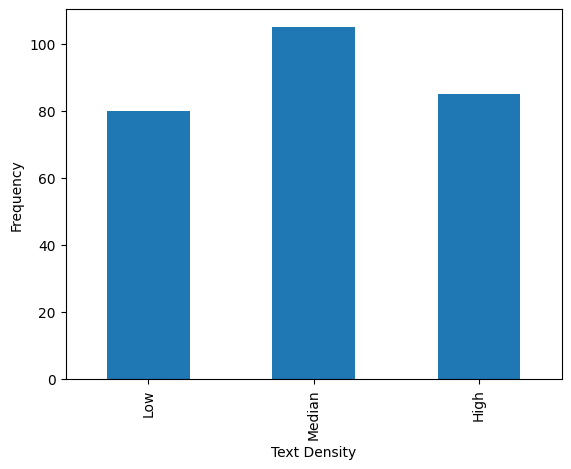
\includegraphics[width=0.75\linewidth]{distexperiment4.png}
    \caption{The distributions of responses of Experiment (2)}
    \label{fig:DistExperiment4}
\end{figure}

\subsubsection{Experiment (3)}
Additional experiments were conducted to cross-validate the findings regarding Hypothesis 2. In this experiment, we only take two levels of text density (i.e., low-level vs high-level). The distributions of the responses are shown in Table \ref{tab: DistExperiment5}. It is shown that images with high-level text density are less preferable. The Chi-square value of the contingency table is 30.09, p<0.01. A summary of the distributions of the responses is shown in Figure \ref{fig:DistExperiment5}.


\begin{table}
\caption{The distributions of responses of Experiment (3)}
\label{tab: DistExperiment5}
\centering

\begin{tabular}{l c c }
\hline
\textbf{Item} & \textbf{Low Density} & \textbf{High Density} \\
\hline \\[-1.8ex]
\textbf{Group1} & 40 & 24 \\
\textbf{Group2} & 46 & 18 \\
\textbf{Group3} & 51 & 13 \\
\textbf{Group4} & 50 & 14 \\
\textbf{Group5} & 33 & 31 \\
\textbf{Group6} & 37 & 27 \\
\textbf{Group7} & 51 & 13 \\
\textbf{Group8} & 43 & 21 \\
\textbf{Group9} & 49 & 15 \\
\textbf{Group10} & 52 & 12 \\
\hline \\[-1.8ex]
\end{tabular}

\end{table}

\begin{figure}
    \centering
    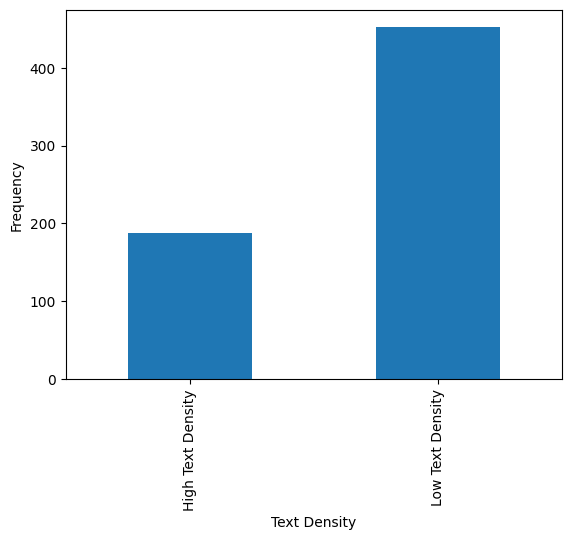
\includegraphics[width=0.75\linewidth]{distexperiment5.png}
    \caption{The distributions of responses of Experiment (3)}
    \label{fig:DistExperiment5}
\end{figure}

\subsubsection{Experiment (4)}
In Experiment (4), we examine the impact of text positions on campaign attractiveness. Based on the results of econometric analysis in the previous section, we can learn that texts in the center position are preferable. Therefore, we take two levels of text positions, $Center$ VS $Other$. A total of 65 students participated in this experiment, with 40 females and 25 males. The distributions of responses are shown in Table \ref{tab: DistExperiment6}. A summary of distributions in shown in Figure \ref{fig:DistExperiment6}.

\begin{table}
\caption{The distributions of responses of Experiment (4)}
\label{tab: DistExperiment6}
\centering

\begin{tabular}{l c c}
\hline
\textbf{Item} & \textbf{Other Position} & \textbf{Center Position} \\
\hline \\[-1.8ex]
\textbf{Group1} & 45 & 20 \\
\textbf{Group2} & 56 & 9 \\
\textbf{Group3} & 48 & 17 \\
\textbf{Group4} & 45 & 20 \\
\textbf{Group5} & 47 & 18 \\
\textbf{Group6} & 52 & 13 \\
\textbf{Group7} & 45 & 20 \\
\textbf{Group8} & 21 & 44 \\
\textbf{Group9} & 47 & 18 \\
\textbf{Group10} & 14 & 5 \\
\hline \\[-1.8ex]
\end{tabular}

\end{table}
\begin{figure}
    \centering
    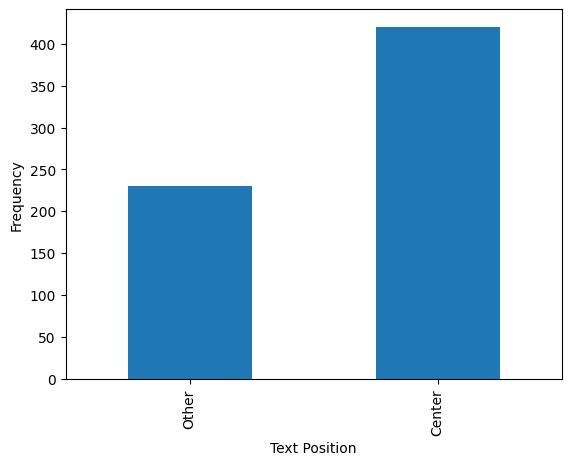
\includegraphics[width=0.75\linewidth]{distexperiment6.png}
    \caption{The distributions of responses of Experiment (4)}
    \label{fig:DistExperiment6}
\end{figure}



\section{Discussions}
\section{Conclusions}
Here is the conclusion.
\printbibliography
\end{document}
